\chapter{2018年「大学物理2」\titlelogo{https://sci.hdu.edu.cn}{HDU}期末试题}
\date{2019年1月15日}{大学物理教学团队}{A0715012}
{未央物理讲师 \href{https://qm.qq.com/q/UPbGudx8cK}{\textbf{Axia}}}
{https://h5.qun.qq.com/s/WRps3LNC8K}{HDU 物理营}
{http://weixin.qq.com/r/mhKYgFTEMQlOrRDj90eI}{未央学社公众号}

\section{选择题（每题3分，共27分）}
\begin{choice}{C}[简谐振动]
    一质点做简谐振动，周期为$T$. 当它由平衡位置向$x$轴正方向运动时，从二分之一最大位移处到最大位移处这段路程所需要的时间为
    \begin{tasks}(4)
        \task $\frac{T}{12}$
        \task $\frac{T}{8}$
        \task $\frac{T}{6}$
        \task $\frac{T}{4}$
    \end{tasks}
\end{choice}
\solute2
\begin{solution}*
    $\Delta t=\Delta\varphi/\omega=\pi/3\omega\xlongequal{\omega=2\pi/T}T/6$. \sokka{C}
\end{solution}

\vskip-2ex
\begin{paracol}{2}
\begin{choice}{A}[平面简谐波的波函数]
    一平面简谐波沿$Ox$轴正方向传播. $t=0$时刻的波形图如图所示，则$P$处介质质点的振动方程为
    \begin{tasks}(2)
        \task $y_p=0.10\cos{\ab(4\pi t+\pi/3)}$
        \task $y_p=0.10\cos{\ab(4\pi t-\pi/3)}$
        \task $y_p=0.10\cos{\ab(2\pi t+\pi/3)}$
        \task $y_p=0.10\cos{\ab(2\pi t+\pi/6)}$
    \end{tasks}
\end{choice}
\switchcolumn\centering
\vfill
    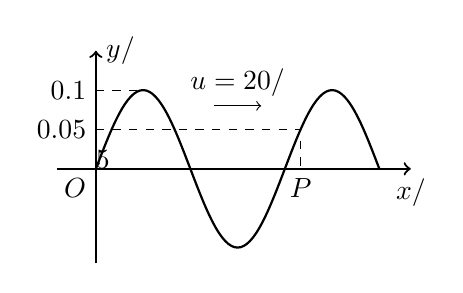
\begin{tikzpicture}
        \draw [thick,->] (-0.5,0)--(4,0) node [anchor=north] {$x/\unit{\m}$};
        \draw [thick,->] (0,-1.2)--(0,1.5) node [anchor=west] {$y/\unit{\m}$};
        \draw [thick] (0,0) sin (0.6,1) cos (1.2,0) sin (1.8,-1) cos (2.4,0) sin (3,1) cos (3.6,0);
        \node [anchor=north east] at (0,0) {$O$};
        \draw [dashed] (0,0.5)--(2.6,0.5) node [anchor=east,at start] {$0.05$} --(2.6,0) node [anchor=north] {$P$};
        \draw [dashed] (0,1)--(0.6,1) node [anchor=east,at start] {$0.1$};
        \draw [->] (1.5,0.8)--(2.1,0.8) node [anchor=south,midway] {$u=\qty{20}{\m/\s}$};
        \length{(0,-0.25)}{(1.2,-0.25)}{$\qty{5}{\m}$}{(0.5,0)}
    \end{tikzpicture}
\vfill
\end{paracol}
\vspace{-.75em}
\solute2
\begin{solution}*
    $\omega=2\pi u/\lambda=4\pi$，$P$处相位$\varphi=\pi/3$. 所以振动方程$y_p=0.10\cos{\ab(4\pi t+\pi/3)}$. \sokka{A}
\end{solution}

\begin{choice}{B}[光的偏振]
    两偏振片堆叠在一起，一束\textbf{自然光}垂直入射其上时没有光线通过. 当其中一偏振片慢慢转动$180^{\circ}$时透射光强度发生的变化为
    \begin{tasks}(2)
        \task 光强单调增加
        \task 光强先增加，后又减小至零
        \task 光强先增加，后减小，再增加
        \task 光强先增加，然后减小，再增加，再减小至零
    \end{tasks}
\end{choice}
\begin{solution}*
    两偏振片由正交到平行再到正交，由Malus定律可知透射光强先增加再减小至零. \sokka{B}
\end{solution}

\begin{choice}{D}[光程与光程差]
    在真空中波长为$\lambda$的单色光，在折射率为$n$的透明介质中从$A$沿着某路径传播到$B$，若$A$、$B$两点相位差为$3\pi$，则此路径$AB$的光程差为
    \begin{tasks}(4)
        \task $3\lambda$
        \task $1.5\lambda/n$
        \task $1.5n\lambda$
        \task $1.5\lambda$
    \end{tasks}
\end{choice}
\solute1
\begin{solution}*
    由$\Delta\varphi=2\pi\delta/\lambda$得$\delta=\lambda\Delta\varphi/2\pi=1.5\lambda$. \sokka{D}\hfill【$AB$的距离为$\overline{AB}=\delta/n=1.5\lambda/n$】
\end{solution}

\begin{choice}{B}[双缝干涉]
    在双缝干涉实验中，为使屏上的干涉条纹间距变大，可采取的办法是
    \begin{tasks}(4)
        \task 使屏靠近双缝
        \task 使两缝的间距变小
        \task 把两缝的宽度调窄
        \task 改用波长短的单色光
    \end{tasks}
\end{choice}
\begin{solution}*
    已知双缝干涉条纹间距公式$\Delta x=\lambda L/d$. 要使$\Delta x$变大，可增大波长$\lambda$、屏幕与双缝的距离$L$或减小双缝间距$d$. \sokka{B}
\end{solution}

\vskip-2ex
\begin{paracol}{2}
    \begin{choice}{D}[弗琅禾费衍射]
        一束波长为$\lambda$的平行单色光垂直入射到单缝$AB$上，装置如图. 在屏幕$D$上形成衍射图样，如果$P$是中央亮纹一侧一级暗纹，则$\overline{BC}$的长度为
    \begin{tasks}(4)
        \task $\lambda/2$
        \task $2\lambda$
        \task $3\lambda/2$
        \task $\lambda$
    \end{tasks}
    \end{choice}
    \switchcolumn\centering
\vfill
\begin{tikzpicture}
    \filldraw [fill=gray] (0.2,1.5) rectangle (0,0.5) node [anchor=south east] {$A$};
    \filldraw [fill=gray] (0.2,-1.5) rectangle (0,-0.5) node [anchor=north east] {$B$};
    \draw [thick,dashed] (-1.2,0)--(3.6,0);
    \draw [thick] (3.6,1.5)--(3.6,-1.5) node [anchor=west,at start] {$D$} node [anchor=west] {屏};
    \filldraw [fill=backgroundcolor] (1.5,0) ellipse (0.1 and 1.2);
    \foreach \y in {0.5,0,-0.5}
    \draw [thick,->,yshift=\y cm] (-1,0)--(0,0);
    \length{(1.5,-1.4)}{(3.6,-1.4)}{$f$}{(0.25,0)}
    \node [anchor=south] at (-1,0.5) {$\lambda$};
    \node [anchor=south] at (1.5,1.2) {$L$};
    \draw [thick] (0,0.5)--(1.5,1)--(3.6,1);
    \draw [thick] (0,0)--(1.5,0.5)--(3.6,1);
    \draw [thick] (0,-0.5)--(1.5,0)--(3.6,1) node [anchor=west] {$P$};
    \draw [dashed] (0,-0.5)--(0,0.5)--(0.32,-0.4) node [anchor=north west] {$C$};
\end{tikzpicture}
\vfill
\end{paracol}
\vspace{-.75em}
\solute1
\begin{solution}*
    由暗纹条件$\overline{BC}=\delta=1\cdot\lambda$. \sokka{D}
\end{solution}

\begin{choice}{A}[钟慢效应]
    静止于某地的甲测得该地发生两件事时间间隔为$\qty{4}{\s}$，若另一惯性系的乙测得时间间隔为$\qty{5}{\s}$，则乙相对甲的速度是
    \begin{tasks}(4)
        \task $0.6c$
        \task $0.8c$
        \task $0.4c$
        \task $0.2c$
    \end{tasks}
\end{choice}
\solute1
\begin{solution}*
    由钟慢效应公式$\qty{5}{\s}=4/\sqrt{1-v^2/c^2}\unit{\s}$得$v=0.6c$. \sokka{A}
\end{solution}

\begin{choice}{C}[氢原子能级]
    由氢原子理论知，当大量氢原子处于$n=3$的激发态时，原子越迁将发出
    \begin{tasks}(4)
        \task 一种波长的光
        \task 两种波长的光
        \task 三种波长的光
        \task 连续光谱
    \end{tasks}
\end{choice}
\solute1
\begin{solution}*
    氢原子从在$n=1,2,3$中任意两能级间跃迁，即$\mathrm{C}_3^2=3$. \sokka{C}
\end{solution}

\begin{choice}{A}[量子初步]
    粒子在一维无限深方势阱中运动，波函数为$\psi\ab(x)=\frac{1}{\sqrt{{a}}}\cdot\cos{\frac{3\pi x}{2a}}\ (\abs{x}\leq a)$. 则粒子在$x=\frac56a$出现的概率密度为
    \begin{tasks}(4)
        \task $1/2a$
        \task $1/a$
        \task $1/\sqrt{2a}$
        \task $1/\sqrt{a}$
    \end{tasks}
\end{choice}
\solute1
\begin{solution}*
    概率密度$\omega(5a/6)=\abs{\psi(5a/6)}^2=1/2a$. \sokka{A}
\end{solution}

\section{填空题（共21分）}
\begin{problem}[弹簧振子][3]
    质量$M=\qty{1.2}{\kg}$的物体挂在一个轻弹簧上振动，用秒表测得此系统在$\qty{45}{\s}$内震动了$90$次，若在此弹簧上再加挂质量$m=\qty{0.6}{\kg}$的物体，而弹簧所受的力未超过弹性限度，则该系统新的振动周期为\ans{$\qty{0.612}{\s}$}.
\end{problem}
\begin{solution}*
    由$T=2\pi\sqrt{\frac{m}{k}}=\qty{0.5}{\s}$得$T^{\prime}=\sqrt{\frac{M+m}{M}}T=\qty{0.612}{\s}$.
\end{solution}

\begin{problem}[简谐波][3]
    一声波在空气中的波长是$\qty{0.25}{\m}$，传播速度是$\qty{340}{\m/\s}$. 当它进入另一介质时，波长变成了$\qty{0.37}{\m}$. 它在该介质中传播速度为\ans{$\qty{503.2}{\m/\s}$}.
\end{problem}
\begin{solution}*
    由$u=\lambda f$得$u^{\prime}=\lambda'u/\lambda=\qty{503.2}{\m/\s}$.
\end{solution}

\begin{problem}[迈克尔逊干涉仪][3]
    在迈克尔逊干涉仪的一条光路中，垂直于光路放入折射率为$n$、厚度为$h$的透明介质薄膜. 与未放入此薄膜时相比较，两光束光程差的改变量为\ans{$2\ab(n-1)h$}.
\end{problem}
\begin{solution}*
    迈克尔逊干涉仪光路上的某点光碰到反射镜后会再次经过此处，故原来的光程为$2h$；现在加入了透明薄片，使得这里的光程为$2nh$，故光程差为$2\ab(n-1)h$.
\end{solution}

\begin{problem}[光栅][3]
    某单色光垂直入射到一个每毫米有$800$条线的光栅上. 如果第一级谱线的衍射角为$30^{\circ}$，则入射光的波长为\ans{$\qty{625}{\nm}$}.
\end{problem}
\begin{solution}*
    光删常数$d=1/800=\qty{1.25}{\um}$，由$d\sin{30^{\circ}}=1\cdot\lambda$得$\lambda=\qty{625}{\nm}$.
\end{solution}

\begin{problem}[光的偏振][3]
    使光强为$I_0$的自然光依次垂直通过偏振片$P_1,\ P_2$和$P_3$. $P_1$与$P_2$的偏振化方向成$45^{\circ}$角，$P_2$与$P_3$的偏振化方向成$45^{\circ}$角. 则透过三块偏振片的光强$I$为\ans{$I_0/8$}.
\end{problem}
\solute0
\begin{solution}*
    由Malus定律得$I=(1/2)\times I_0\cos^2{45^{\circ}}\cos^2{45^\circ}=I_0/8$.
\end{solution}

\begin{problem}[相对论能动量关系][3]
    质子在加速器中被加速，当其动能为静止能量的$3$倍时，其质量为静止质量的\ans{$4$}倍.
\end{problem}
\solute0
\begin{solution}*
    由题意$E_k=mc^2-m_0c^2=3m_0c^2$得$m=4m_0$.
\end{solution}

\begin{problem}[de Broglie波][3]
    在$B=\qty{1.25e-2}{\T}$的匀强磁场中沿半径$R=\qty{1.66}{\cm}$的圆轨道运动的$\alpha$粒子的de Broglie波长是\ans{$\qty{0.0997}{\AA}$}.
\end{problem}
\begin{solution}*
    由$2evB=\frac{mv^2}{R}$得$v=\frac{2eBR}{m}$. $\lambda=\frac{h}{p}=\frac{h}{mv}=\frac{h}{2eBR}=0.0997\text{\AA}$.
\end{solution}

\section{计算题（共52分）}
\begin{problem}[简谐振动的合成][5]
    一物体同时参与两个同方向的简谐振动
    \[x_1=0.04\cos{\ab(2\pi t+\frac{1}{2}\pi)},\ x_2=0.03\cos{\ab(2\pi t+\pi)}\]

    求此物体的振动方程.
\end{problem}
\solute1
\begin{solution}
\begin{itemize}
\begin{multicols}{2}
    \item 合相位$\varphi=\pi+\frac{A_1\sin{\varphi_1}+A_2\sin{\varphi_2}}{A_1\cos{\varphi_1}+A_2\cos{\varphi_2}}=127^{\circ}$\point{2}
    \item 合振幅$A=\sqrt{A_1^2+A_2^2+2A_1A_2\cos{\varphi}}=0.05$\point{2}
\end{multicols}
\item 振动方程为$x=0.05\cos{\ab(2\pi t+127^{\circ})}$\point{1}
\end{itemize}
\end{solution}

\begin{problem}[驻波][8]
两波在一很长的弦上传播，其表达式分别为$y_1=4\times 10^{-2}\cos{\ab[\frac{1}{3}\pi\ab(4x-24t)]},\ y_2=4\times 10^{-2}\cos{\ab[\frac{1}{3}\pi\ab(4x+24t)]}$. 求
    \begin{enumerate}
        \item 两波的频率、波长、波速.
        \item 两波叠加后的节点位置.
        \item 叠加后振幅最大的那些点的位置.
    \end{enumerate}
\end{problem}
\solute0
\begin{solution}
\begin{enumerate}
    \item $\omega_1=\omega_2=8\pi\unit{s^{-1}},\ \nu_1=\nu_2=4\unit{s^{-1}}$.\point{2}
    \item 驻波表达式$y=y_1+y_2=8\times 10^{-2}\cos{\ab(8\pi t)}\cos{\ab(\frac{4\pi x}{3})}\point{2}$

    波节的位置$\cos{\ab(\frac{4\pi x}{3})}=0,\ x=\frac{6k+3}{8},\ k=0,1,2,\cdots$.\point{2}

    \item 振幅最大点即波腹的位置$\cos{\ab(\frac{4\pi x}{3})}=\pm 1,\ x=\frac{3k}{4},\ k=0,1,2,\cdots$. \point{2}
\end{enumerate}
\end{solution}

\begin{problem}[光栅][8]
    波长$\lambda=\qty{600}{\nm}$的单色光垂直入射到一光栅上，第二级主极大衍射角为$30^{\circ}$，第三级缺级.
    \begin{enumerate}
        \item 光栅常数$d=a+b$等于多少？
        \item 透光缝可能的最小宽度$a$等于多少？
        \item 在上述$d$和$a$值下，求在衍射角$-\frac{1}{2}\pi<\varphi<\frac{1}{2}\pi$范围内可观察到的全部主级大的级次.
    \end{enumerate}
\end{problem}
\solute0
\begin{solution}
    \begin{enumerate}
        \item 由光栅方程$(a+b)\sin30^\circ=2\lambda$得$d=\frac{2\lambda}{\sin{30^{\circ}}}=\qty{2.4}{\um}$. \point{2}
        \item 由缺级条件$k=k'\frac{d}{a}$得$a=(a+b)/3=\qty{0.8}{\um}$. \point{2}
        \item 取$\varphi=\pm 90^\circ$得$k=\pm4$. 由于$\varphi$无法取到$\pm 90^\circ$，所以$k_{\max}=\pm 3$. \point{2}
        
        由于$\pm 3$级缺级，所以此范围内可见主极大级次为$k=0,\ \pm 1,\ \pm2$. \point{2}
    \end{enumerate}
\end{solution}

\begin{problem}[双缝干涉][5]
    在双缝干涉实验中所用单色光的波长为$\qty{600}{\nm}$，双缝间距为$\qty{1.2}{\mm}$，双缝与屏相距$\qty{500}{\mm}$. 求相邻干涉明纹间距.
\end{problem}
\begin{solution}*
    $\Delta x=\frac{\lambda D}{d}=\qty{0.25}{\mm}$. \point{5}
\end{solution}

\begin{problem}[牛顿环][8]
    牛顿环装置透镜凸表面的曲率半径是$R=\qty{400}{\cm}$. 用某单色平行光垂直入射，观察反射光形成的牛顿环，测得第5个明环的半径是$\qty{0.30}{\cm}$.
    \begin{enumerate}
        \item 求入射光的波长.
        \item 求以透镜中心为圆心在半径为$\qty{1}{\cm}$的范围内可观察到的明环数目.
    \end{enumerate}
\end{problem}
\solute0
\begin{solution}
    \begin{enumerate}
    \item 由明环半径公式$r_k=\sqrt{\frac{\ab(2k-1)\lambda R}{2}}$得入射光的波长$\lambda=\frac{2r^2}{\ab(2k-1)R}=\qty{500}{\nm}$. \point{5}
    \item 由明环半径公式，代入$r=\qty{1}{\cm}$得$k=\left\lfloor\frac{r^2}{\lambda R}+\frac{1}{2}\right\rfloor=50$. \point{3}
    \end{enumerate}
\end{solution}

\begin{problem}[起偏角][5]
    一束自然光自水中入射到空气界面上，若水的折射率为$1.33$，空气的折射率为$1$，求Brewster角.
\end{problem}
\begin{solution}*
    $\theta_B=\arctan{\frac{n_2}{n_1}}=\arctan{\frac{1}{1.33}}=37^{\circ}$. \point{5}
\end{solution}

\begin{problem}[尺缩效应，质速关系][5]
    一体积为$V_0$，静止质量为$m_0$的立方体沿其一棱的方向相对于观察者$A$以速度$v$运动. 求观察者$A$测得其密度.
\end{problem}
\begin{solution}*
    由尺缩效应和质速关系得观察者测得密度为$\rho=\frac{m}{V}=\frac{m_0/\sqrt{1-\beta^2}}{V_0\sqrt{1-\beta^2}}=\frac{m_0}{V_0\ab(1-v^2/c^2)}$. \point{5}
\end{solution}

\begin{problem}[光电效应][8]
    光电管的阴极用逸出功$A=\qty{2.2}{\electronvolt}$的金属制成，今用一单色光照射此光电管，阴极发射出光电子，测得遏止电势差为$\abs{U_a}=\qty{5.0}{\electronvolt}$. 试求
\begin{enumerate}
    \item 光电管的阴极金属的光电效应红限波长.
    \item 入射光波长.
\end{enumerate}
\end{problem}
\begin{solution}
\begin{enumerate}
    \item 由$E=\frac{hc}{\lambda}-A=0$得红限波长为$\lambda_{\max}=\frac{hc}{A}=\qty{563.56}{\nm}$. \point{4}
    \item 由$eU_a=\frac{hc}{\lambda}-A$得入射光波长$\lambda=\frac{hc}{eU_a+A}=\qty{172.20}{\nm}$. \point{4}
\end{enumerate}
\end{solution}


\vfill
\rightline{/*Powered by \pkg{LiteSolution} \textsf\LaTeX~Template. Designed by WeYoung \href{https://ctan.org/home/xiamyphys}{Axia}.*/}